\documentclass{article}
\usepackage[left=0.5in,top=0.5in,right=0.5in,bottom=0.5in]{geometry}
\usepackage[english]{babel}
\usepackage[utf8]{inputenc}
\usepackage{graphicx}
\usepackage{amssymb,amsmath,amsthm,latexsym}
\graphicspath{{./images/}}
\title{Intermediate Disturbance Hypothesis Lab Report}
\author{Philip Kim}
\date{\today}
\begin{document}
\maketitle
\begin{table}[h!]
  \begin{center}
    \caption{\(Morphospecies_{A,B,C}\)}\label{tab:table1}
    \begin{tabular}{|c|c|c|}\hline
      \(M_{A}\): No disturbance & \(M_{B}\): Mid disturbance & \(M_{C}\): High disturbance \\ \hline
      7 & 13 & 3 \\ \hline
      7 & 9 & 4 \\ \hline
      2 & 4 & 4 \\ \hline
      4 & 4 & 2 \\ \hline
      11 & 14 & 10 \\ \hline
      13 & 14 & 8 \\ \hline
      4 & 10 & 8 \\ \hline
      10 & 7 & 8 \\ \hline
      4 & 7 & 6 \\ \hline
      4 & 7 & 4 \\ \hline
      6 & 5 & 5 \\ \hline
      7 & 6 & 5 \\ \hline
      7 & 3 & 5 \\ \hline
      1 & 5 & 8 \\ \hline
      11 & 15 & 9 \\ \hline
      4 & 9 & 8 \\ \hline
      21 & 15 & 14 \\ \hline
      19 & 14 & 15 \\ \hline
      9 & 13 & 10 \\ \hline
      7 & 14 & 20 \\ \hline
      8 & 11 & 17 \\ \hline
      6 & 10 & 14 \\ \hline
      15 & 12 & 18 \\ \hline
      7 & 11 & 5 \\ \hline
      12 & 15 & 10 \\ \hline
      11 & 14 & 9 \\ \hline
      23 & 30 & 13 \\ \hline
      12 & 7 & 8 \\ \hline
      13 & 20 & 12 \\ \hline
    \end{tabular}
  \end{center}
  \begin{center}
    \begin{equation}
      \begin{split}
        n &= 29 \\
        \overline{x} &= \frac{x_1 + x_2 + \cdots + x_n}{n} \\
        \sigma_{x} &= \sqrt{\frac{{|x_1 - \overline{x}|}^2 + {|x_2 - \overline{x}|}^2 + \cdots + {|x_n - \overline{x}|}^2}{n-1}} \\
        \epsilon_{x} &= \frac{\sigma_{x}}{\sqrt{n}} \\
        \overline{A},~\overline{B},~\overline{C} &= 9.1379, 10.9655, 9.0345 \\
        \sigma_{A},~\sigma_{B},~\sigma_{C} &= 5.4098, 5.5964, 4.7017 \\
        \epsilon_{A},~\epsilon_{B},~\epsilon_{C} &= 0.1865, 0.1930, 0.1621 \\
      \end{split}
    \end{equation}
  \end{center}
\end{table}
\newpage
\begin{center}
  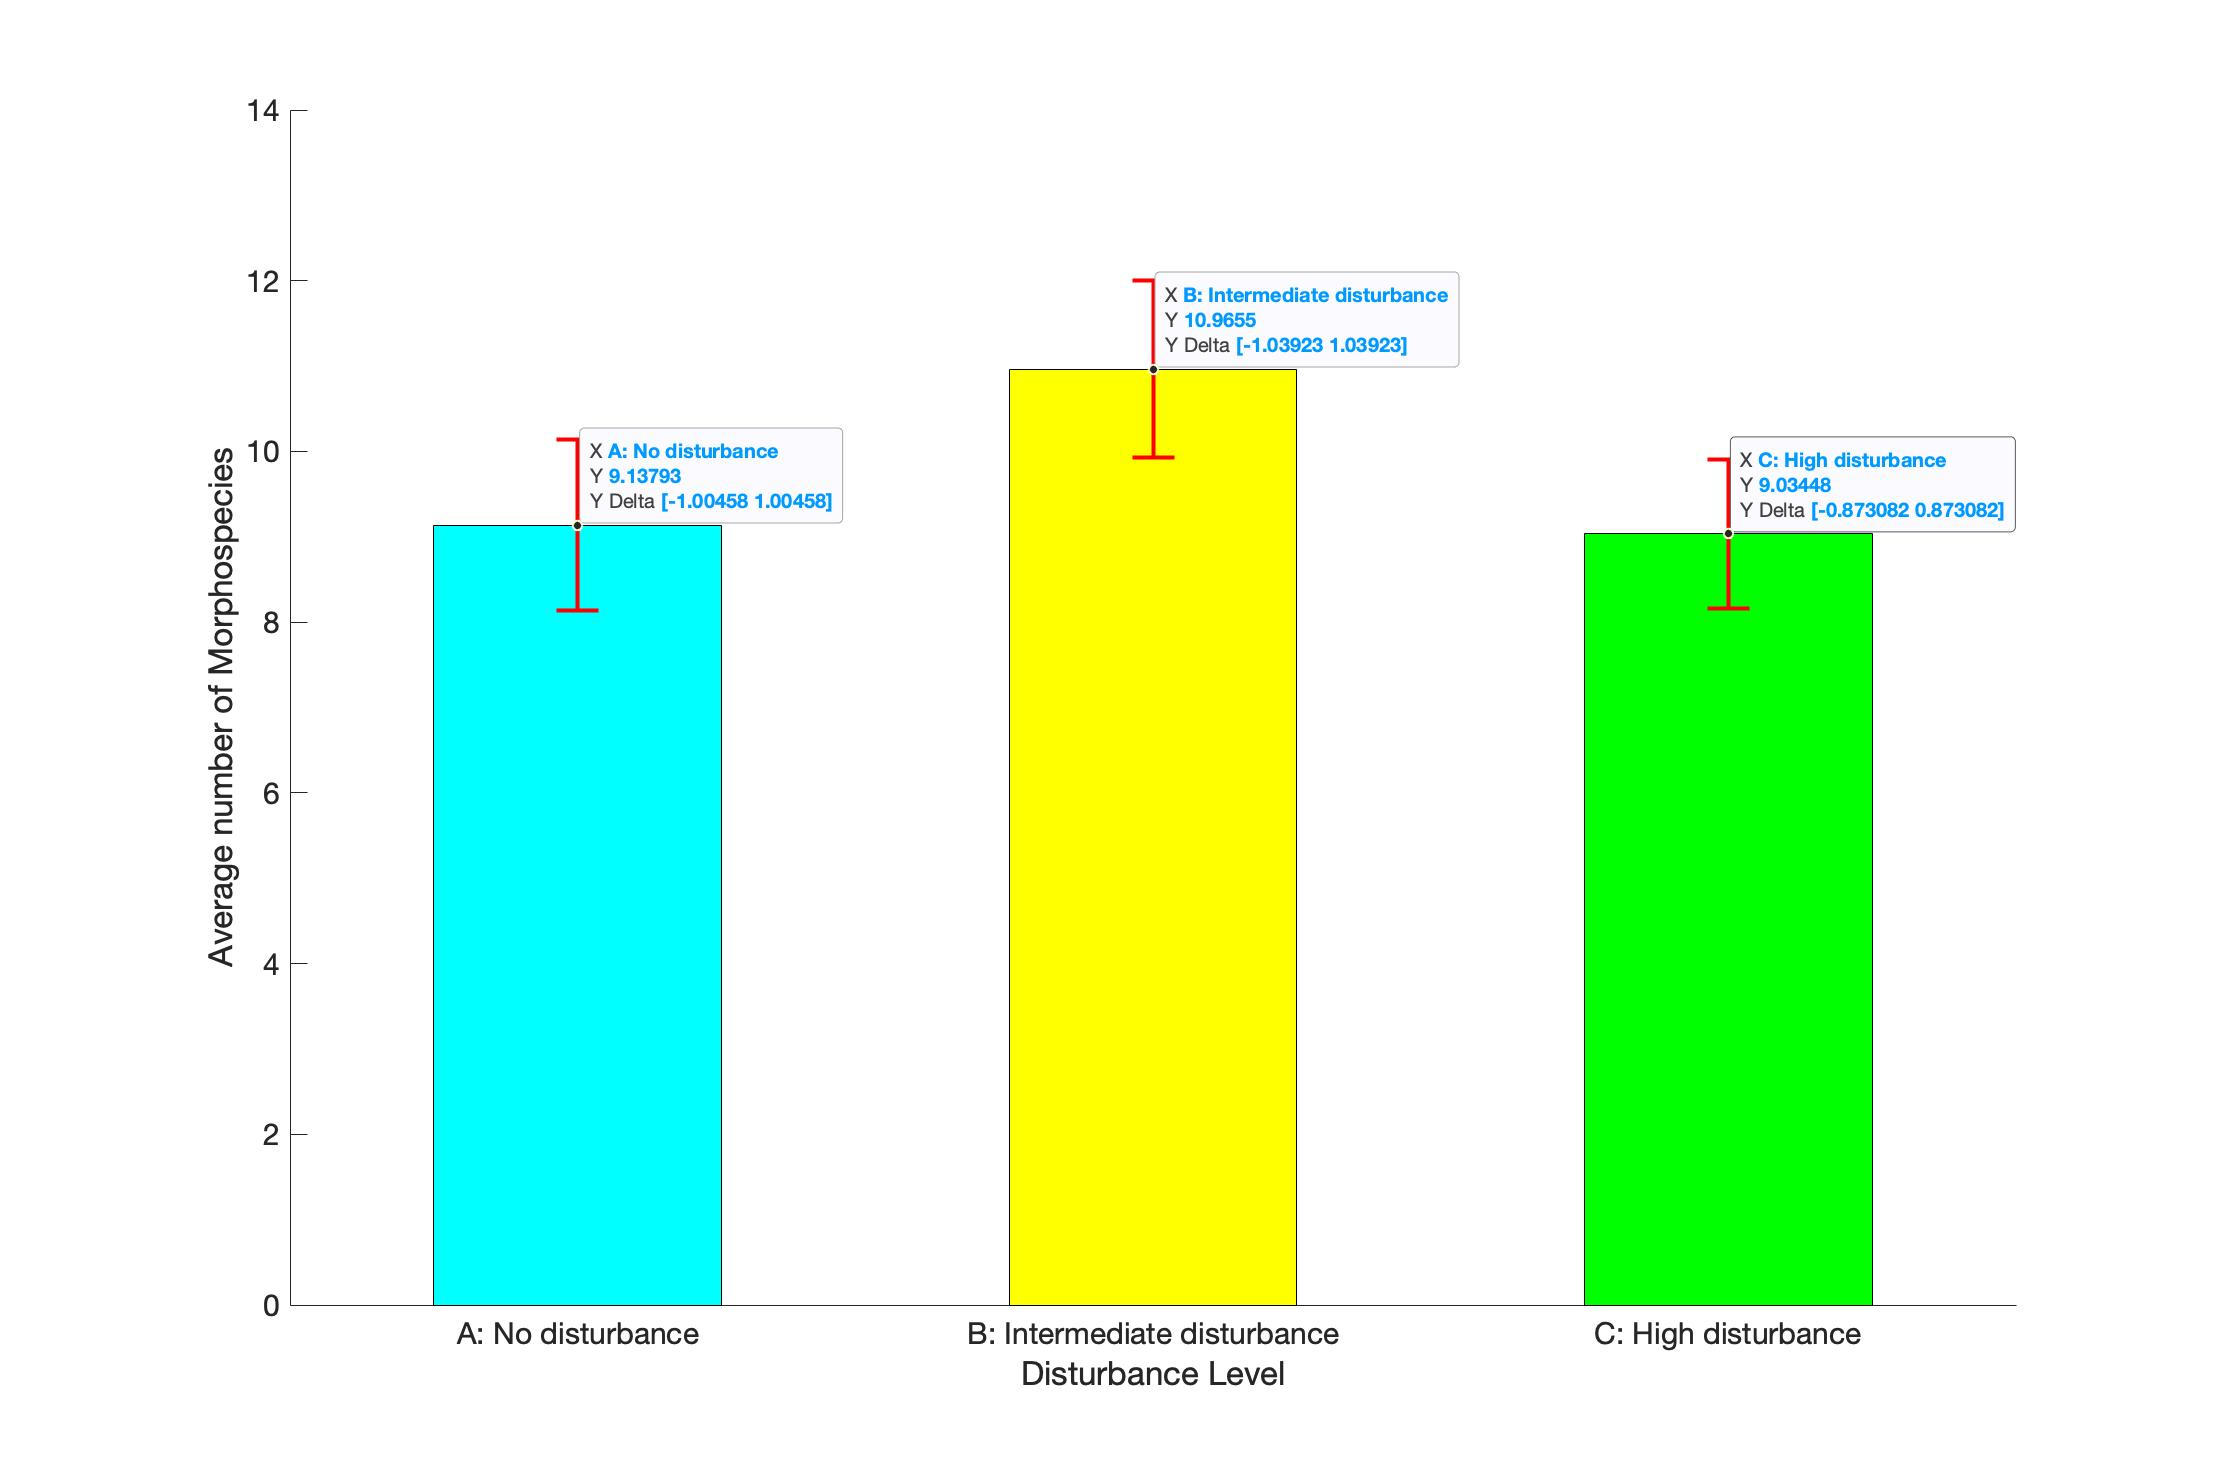
\includegraphics[width=\textwidth]{idh.jpg}
\end{center}
In the bar chart above, are the averages of morphospecies with no disturbance, intermediate disturbance and high disturbance. The error bar for A (no disturbance) has no significant difference compared to C (high disturbance). However, B (intermediate disturbance) has significant difference with both A (no disturbance) and C (high disturbance).
\end{document}